\chapter{Feature Selection}\label{feature_selection}

Among all the information received from CrowdTangle, the "Likes" information related to a post, which denotes the total number of likes was discarded. It was done due to several reasons- 

\begin{enumerate}
    \item {The Facebook News Feed ranking algorithm gives less importance to it.}\cite{fbnews}
    \item {The like count of a post bears no significance. As a reaction, it is treated as a neural one since it is thought to belong to a lower sentimental reaction.}
    \item {The total like count of our collected data amounted to more than the sum of other reactions. As a result, taking it into calculation would nullify the importance of other reactions by a large margin.}
\end{enumerate}

\begin{figure}[H]
    \begin{center}
        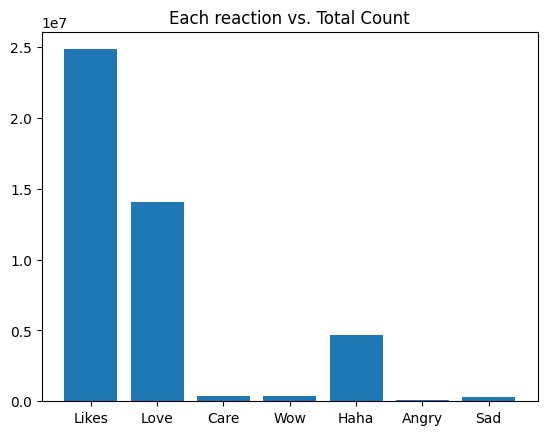
\includegraphics[height=0.5\linewidth]{figures/reaction_distribution.png}
        \caption{Distribution of Different Reactions of Facebook Food Review Posts}
        \label{reaction_count}            
    \end{center}
\end{figure}

In table \ref{reaction_count}, it is quite evident that the total number of likes outperforms all other reactions.

\section{Correlation Coeffiecients}

\begin{figure}[H]
    \begin{center}
        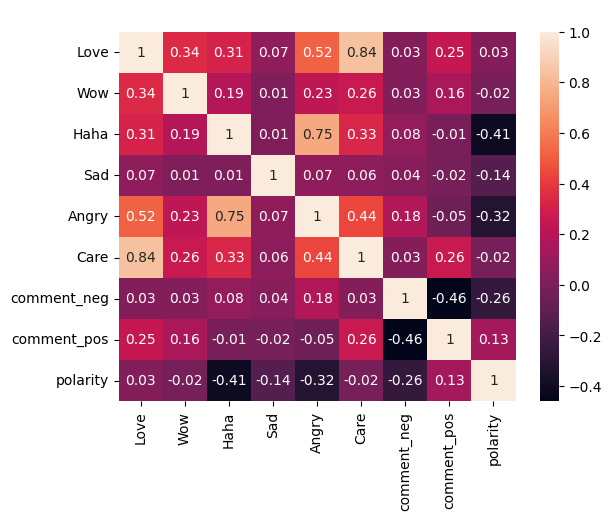
\includegraphics[width=\linewidth]{figures/corr_matrix_reacts.png}
        \caption{Correlation Coefficients of Different Features}
        \label{corr_coeff}
    \end{center}
\end{figure}

Table \ref{corr_coeff} portrays the different correlation coefficients of different features of our dataset. Among them, the value of coefficients between \textbf{Love} and \textbf{Care}, and \textbf{Haha} and \textbf{Angry} are higher than others. It goes on to show that there is a strong correlation between these four reactions. Since the correlation value between them are positive, it means a positive correlation.

\section{Reaction Classes}

As there exists a strong positive correlation between \textbf{Love} and \textbf{Care}, we group them into the positive reaction class. And since \textbf{Haha} and \textbf{Angry} reactions have a positive correlation between them, we group them into the negative reaction class. Since the reactions in social media are disjoint and have no effects on each other, we can not find any negative correlation between the features.

As we had previously discarded \textbf{Like} as a significant reaction, only \textbf{Wow} and \textbf{Sad} remains to be grouped into classes. The reaction \textbf{Wow} is considered to be a positive sentiment. As a result, we put it alongside \textbf{Love} and \textbf{Care} in the positive class. \textbf{Sad} reaction is considered to of a negative sentiment, as a result, we put it in the negative class. Figure \ref{react_classification} shows our classification of the Facebook reactions. Even \textit{Pratama, et al.} \cite{paper_pratama} employed the same classification in their study of special Facebook reactions.

\begin{figure}
    \begin{center}
        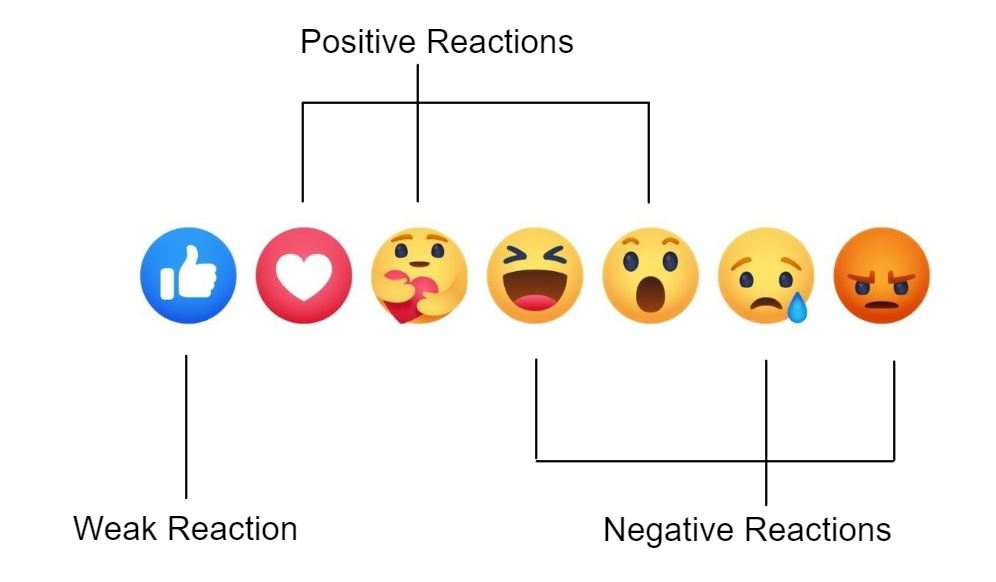
\includegraphics[width=0.6 \linewidth]{figures/react_classification.JPG}
        \caption{Classification of Different Facebook Reactions}
        \label{react_classification}
    \end{center}
\end{figure}

\subsection{Features for interaction Based Method}
Since the interaction-based approach proposed by us in Chapter \ref{methodology} uses a total number of positive and negative reactions, we define two new features from our existing ones. The feature \textit{react\_positive} denotes the total number of reactions belonging to the positive class and the feature \textit{react\_negative} denotes the total number of reactions belonging to the negative class. As a result, we can write down the formula for \textit{polarity} as follows: \

$$  polarity = \frac{n_{positive} - n_{negative}}{n_{positive} + n_{negative}}  $$
$$  n_{positive} = n_{Love} + n_{Care} + n_{Wow}                                $$
$$  n_{negative} = n_{Haha} + n_{Angry} + n_{Sad}                               $$
$$  n_{x}\ =\ Number\ of\ reactions\ for\ reaction\ 'x'\                        $$        

\subsection{Features for Natural Language Processing Method}
Similarly, the same approach is followed for quantifying the features of the Natural Language Processing-based method. In this method, the number of comments belonging to positive and negative classes is computed. It leads to two new features called \textit{comment\_positive} and \textit{comment\_negative} which denotes the total number of positive and negative comments predicted by the fine-tuned BanglaBERT model, as stated in Chapter \ref{methodology}.

$$  comment_{positive} = Total\ number\ of\ positive\ comments\ in\ a\ post\ $$
$$  comment_{negative} = Total\ number\ of\ negative\ comments\ in\ a\ post\ $$

In summary, we can list the features used by our methods as follows:

\begin{enumerate}
    \item {
        \textbf{Features for interaction-based approach}
        \begin{enumerate}
            \item {Total number of positive reactions (Love, Care, Wow)}
            \item {Total number of negative reactions (Haha, Angry, Sad)}
        \end{enumerate}
    }
    \item {
        \textbf{Features for Natural Language Processing based approach}
        \begin{enumerate}
            \item {Total number of positive comments}
            \item {Total number of negative comments}
        \end{enumerate}
    }
    
\end{enumerate}